\section{Resultados de recintos acondicionados}
\subsection{Salas de reunión}
Para el caso de las salas de reunión se obtuvieron los siguientes resultados de ambas propuesta de acondicionamiento. (ver tabla ...)
\begin{figure}[H]
    \centering
    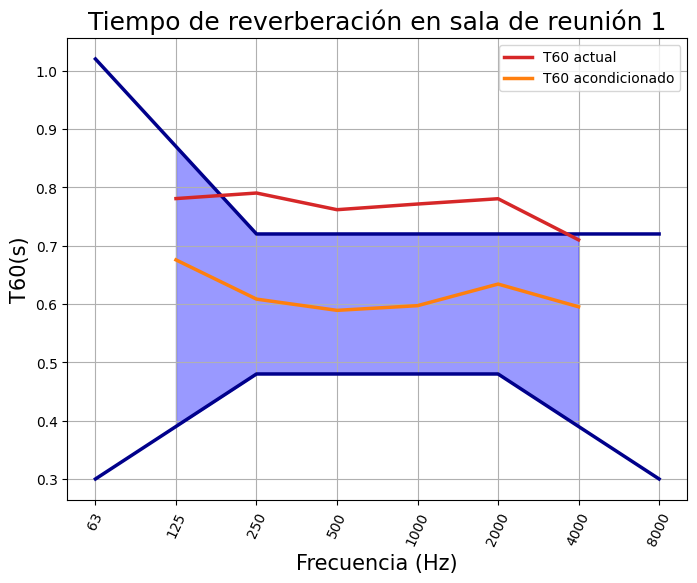
\includegraphics[width=10cm]{Imagenes/DIN/DIN sala reunion 1 comparacion.png}
    \caption{Tiempo de reverberación del estado actual y acondicionado de la sala de reunión 1}
    \label{fig: Ttarger sala_reunion 1 acond}
\end{figure}
\begin{figure}[H]
    \centering
    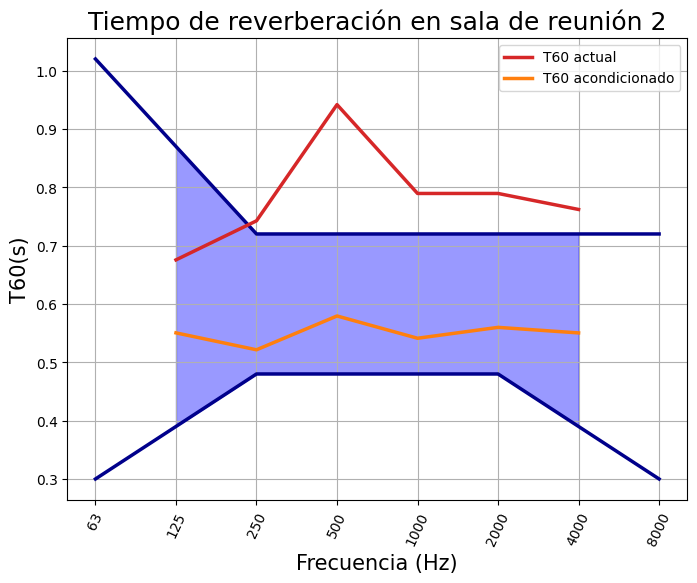
\includegraphics[width=10cm]{Imagenes/DIN/DIN sala reunion 2 comparacion.png}
    \caption{Tiempo de reverberación del estado actual y acondicionado de la sala de reunión 2}
    \label{fig: Ttarger sala_reunion 2 acond}
\end{figure}

\begin{table}[H]
    \resizebox{\textwidth}{!}{%
    \begin{tabular}{|l|l|ll|ll|}
    \hline
     &  & \multicolumn{2}{l|}{\textbf{Sala de reunión 1}} & \multicolumn{2}{l|}{\textbf{Sala de reunión 2}} \\ \cline{3-6} 
    \multirow{-2}{*}{\textbf{Parámetro}} & \multirow{-2}{*}{\textbf{Recomendación}} & \multicolumn{1}{l|}{\textbf{Estado actual}} & \textbf{Propuesta} & \multicolumn{1}{l|}{\textbf{Estado actual}} & \textbf{Propuesta} \\ \hline
    $T_{target}$ & $0.6$ & \multicolumn{1}{l|}{\textcolor{red}{No cumple}} & \textcolor{teal}{Cumple} & \multicolumn{1}{l|}{\textcolor{red}{No cumple}} & \textcolor{teal}{Cumple} \\ \hline
    $C_{50speech}$ & $C_{50speech}>0$ & \multicolumn{1}{l|}{\textcolor{teal}{$1.79$}} & \textcolor{teal}{$3.5$} & \multicolumn{1}{l|}{\textcolor{teal}{$0.89$}} & \textcolor{teal}{$3.9$} \\ \hline
    STI & STI \textgreater $0.45$ & \multicolumn{1}{l|}{\textcolor{teal}{$0.66$}} & \textcolor{teal}{$0.70$} & \multicolumn{1}{l|}{\textcolor{teal}{$0.64$}} & \textcolor{teal}{$0.72$} \\ \hline
    \end{tabular}%
    }
    \caption{Parámetros acústicos de las salas de reunión del estado actual y acondicionado}
    \label{tab: resultados salas de reunion}
\end{table}

\subsection{Sala de ensayo}
\begin{figure}[H]
    \centering
    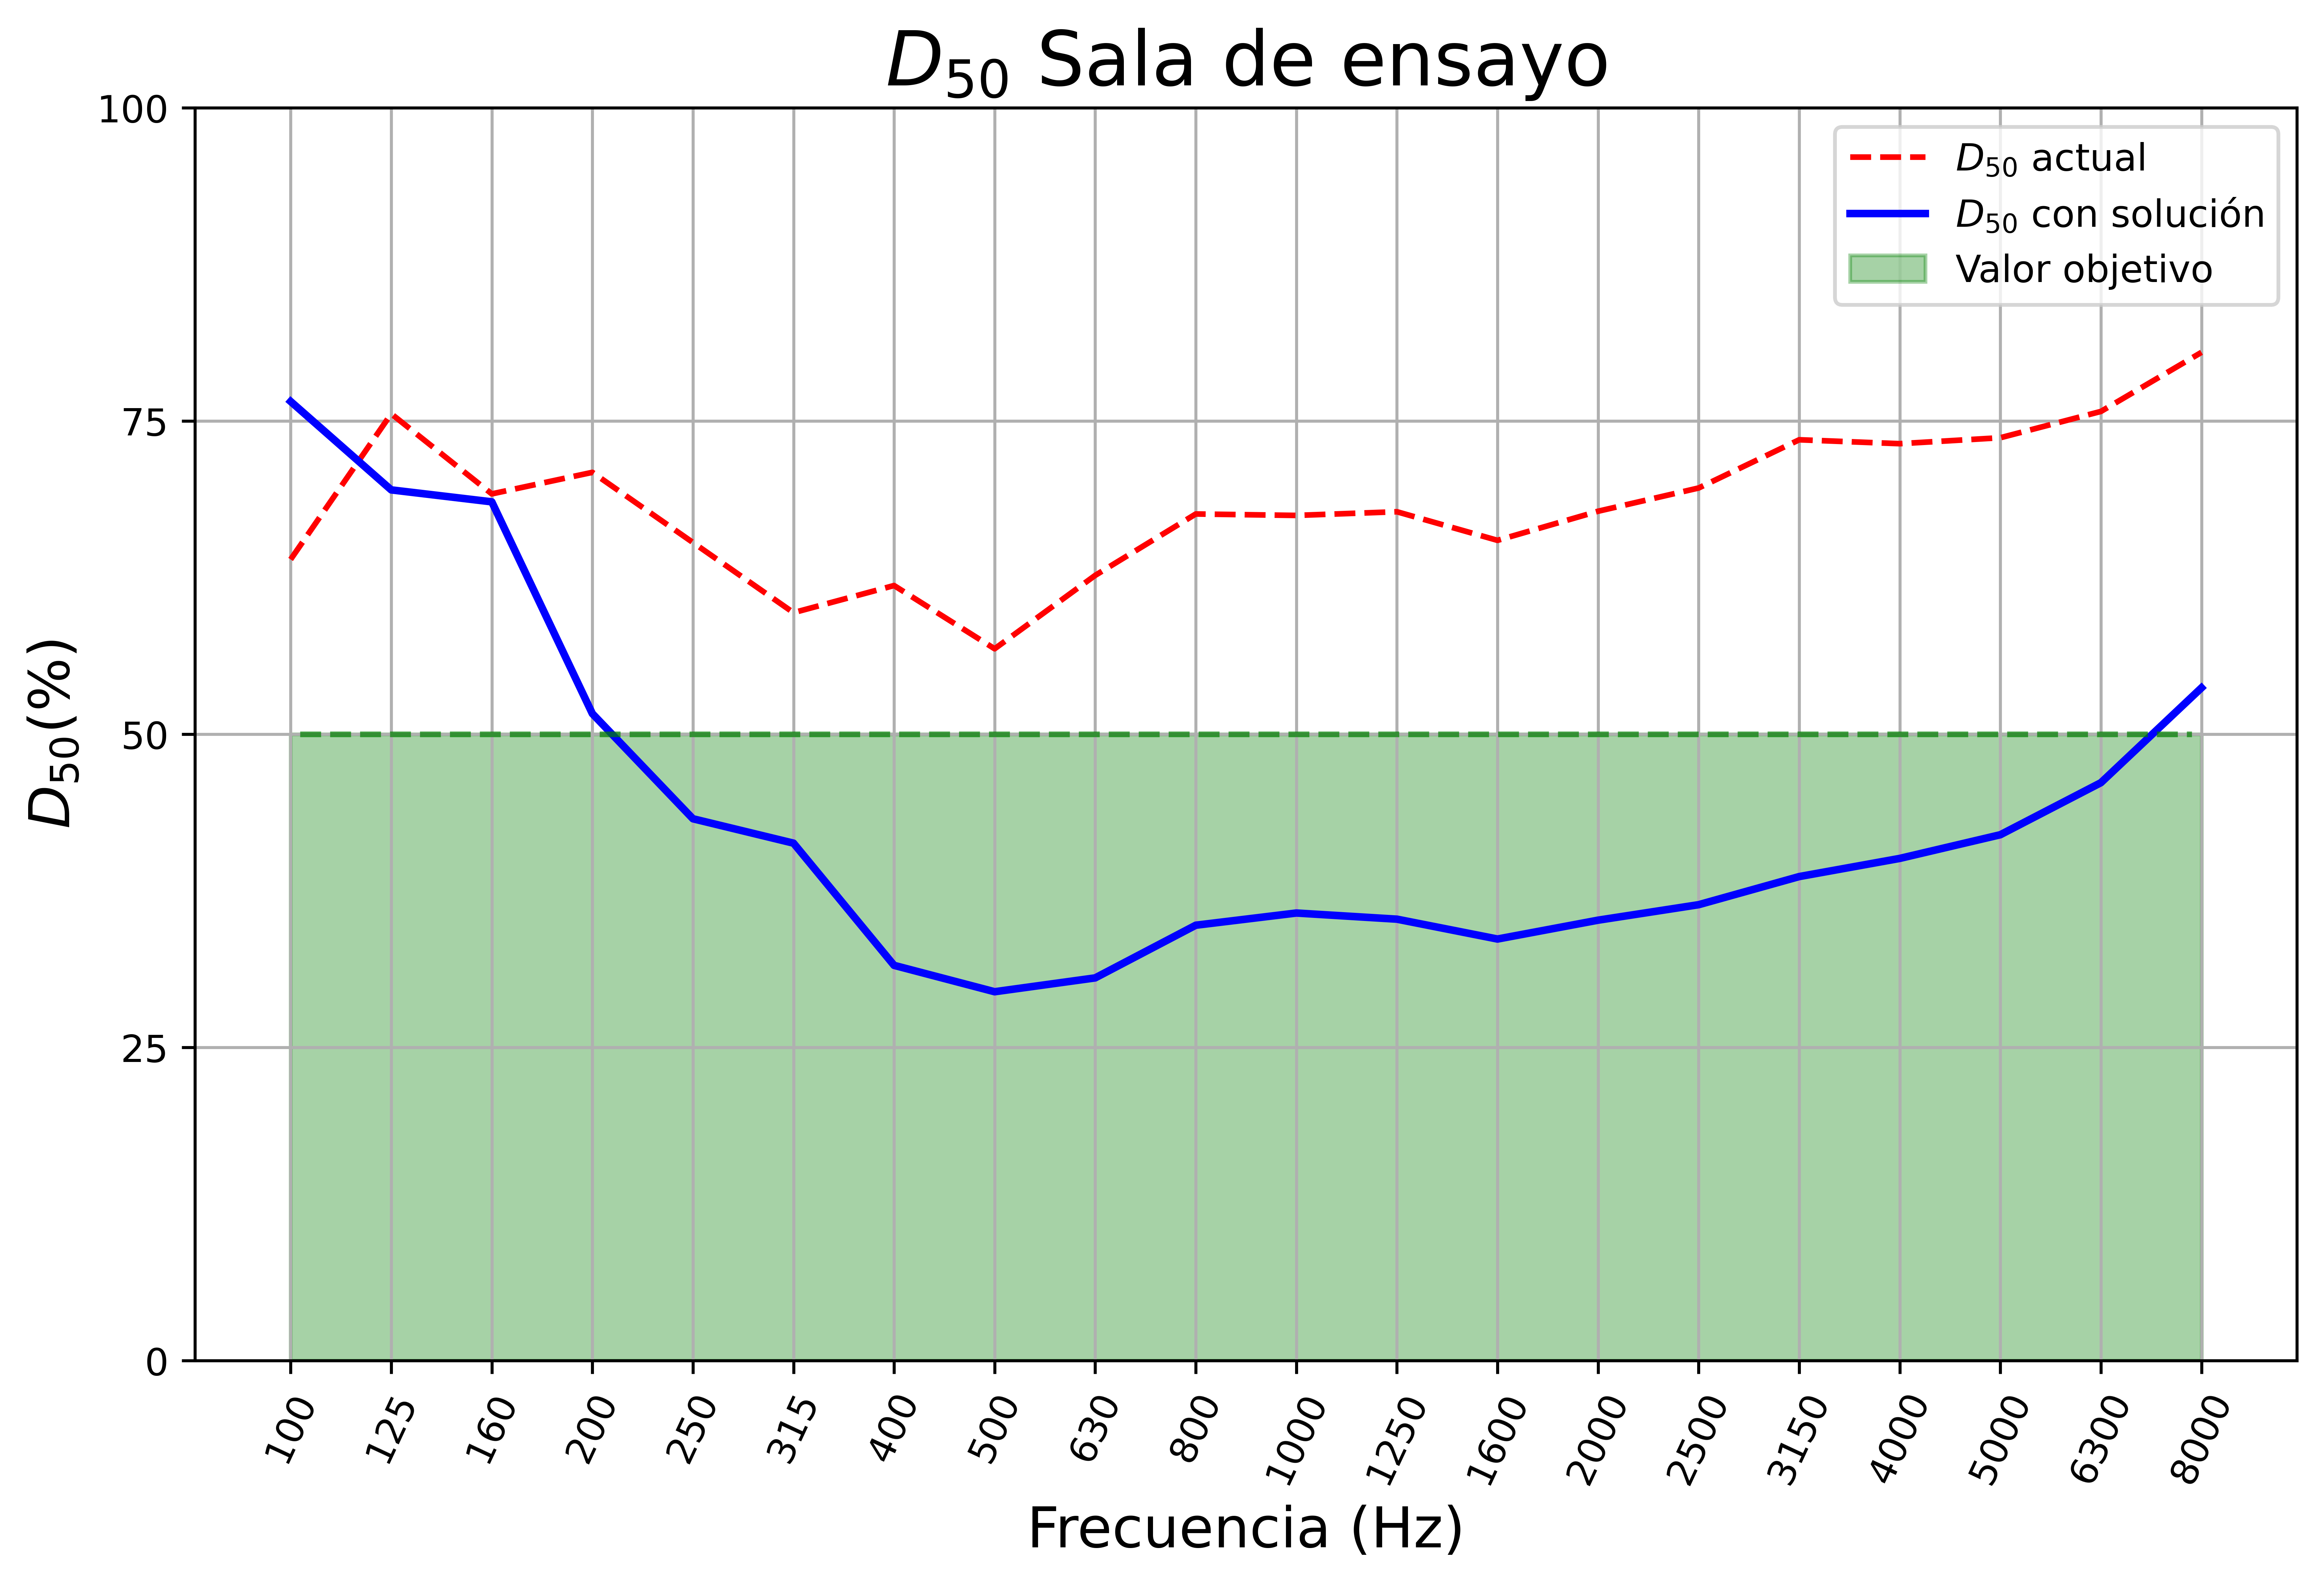
\includegraphics[width=10cm]{Imagenes/Resultados/D50_comparacion.png}
    \caption{$D_{50}$ del estado actual y acondicionado de sala de ensayo}
    \label{fig: D50 de la sala de ensayo acond}
\end{figure}


Para el caso de la sala de ensayo se obtuvieron los siguientes resultados. (ver tabla \ref{tab: resultados sala de ensayo})
\begin{table}[H]
    \centering
    \begin{tabular}{|l|l|ll|}
    \hline
     &  & \multicolumn{2}{l|}{\textbf{Sala de ensayo}} \\ \cline{3-4} 
    \multirow{-2}{*}{\textbf{Parámetro}} & \multirow{-2}{*}{\textbf{Recomendación}} & \multicolumn{1}{l|}{\textbf{Estado actual}} & \textbf{Propuesta} \\ \hline
    $RT_{mid}$ & $0.3$ - $0.7$ & \multicolumn{1}{l|}{\textcolor{red}{$0.74$}} & \textcolor{teal}{$1.4$} \\ \hline
    $C_{80}$ & $-2<C_{80}<2$ & \multicolumn{1}{l|}{\textcolor{red}{$6.04$}} & \textcolor{teal}{$3$} \\ \hline
    $D_{50}$ & $D_{50}$ \textless $0.5$ & \multicolumn{1}{l|}{\textcolor{red}{No cumple}} & \textcolor{red}{No cumple} \\ \hline
    \end{tabular}
    \caption{Parámetros acústicos de la sala de ensayo del estado actual y acondicionado}
    \label{tab: resultados sala de ensayo}
\end{table}